\section{The Paired Audit}
\label{sec:framework}

\subsection{Overview}

CLASP builds two distributions over one observation population for each
country--measurement unit. It takes traceroutes, probe metadata, IP
geolocation and ASN mappings, and cable metadata as inputs. It then extracts
segments, projects feasible corridors, and aggregates paired distributions, as
shown in Fig.~\ref{fig:framework_pipeline}.

Exposure and conditional concentration use different denominators. Exposure
records whether a valid traceroute contains an inter-region feasible corridor.
The paired distributions condition on candidate-bearing segments and describe
how their mass is organized.

\begin{figure*}[t]
  \centering
  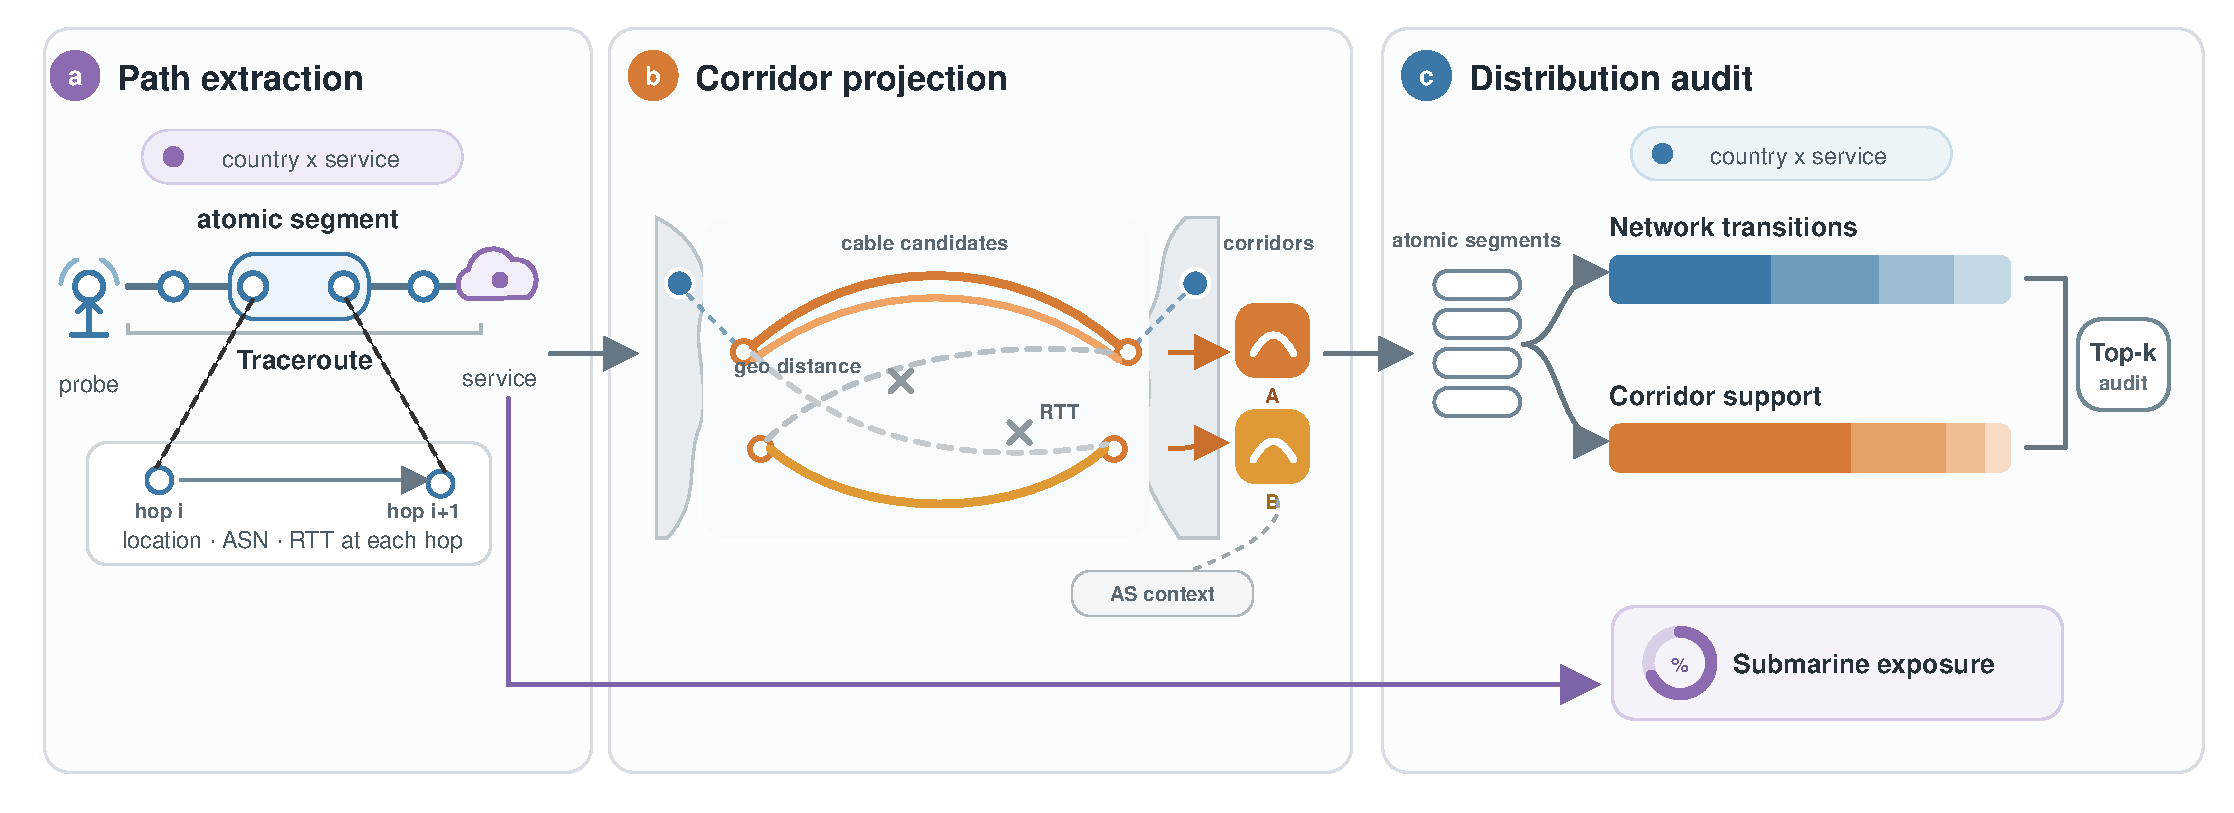
\includegraphics[width=\textwidth]{figures/framework_cross_layer_audit.pdf}
  \caption{CLASP constructs paired network-transition and feasible-corridor
  distributions from candidate-bearing segments in the same observation
  population.}
  \label{fig:framework_pipeline}
\end{figure*}

\subsection{Segments from Service Paths}
\label{sec:framework_segments}

We group traceroutes by probe country and measured service, retaining the
source-side context and the destination selection observed for each
measurement. Hop countries remain segment attributes rather than grouping
keys.

Each traceroute is normalized into its complete sequence of visible hops with
locations, ASNs, and RTTs. Successive visible, geolocated hops form atomic
segments. Each segment records endpoint locations, ASNs, countries, positions,
RTT difference, and bridged-hop count. Repeated hops and RTT samples retain
their trace identity and ordering. When timeouts separate visible hops, the
bridged-hop count records the gap.

When both endpoint ASNs are available, their ordered pair forms the network-
transition label. A segment missing one endpoint ASN receives an ordered
country-pair fallback label. Audit eligibility requires a country-fallback
share of at most 30\%, at least 30 candidate-bearing segments, 10 probes, and
3 probe ASNs.

\subsection{Feasible Corridors}
\label{sec:framework_projection}

For each segment endpoint, we retrieve landing stations within 50~km and pair
them through cable systems in service on July~1, 2026. Explicit cable path or
branch information defines direct landing-point adjacency. When the metadata
does not provide this information, the pipeline retains the candidate at the
topology resolution supplied by the inventory and records that state.

We group landing stations into regions with maximum pairwise distance
30~km. A \emph{landing-region corridor} is a direction-independent pair of
regions connected by at least one feasible cable candidate. Several cable
systems and exact landing pairs can support one corridor, while distinct
coastal entry--exit patterns remain separate.

A candidate must satisfy geographic, lifecycle, and propagation constraints.
Let $D$ be the great-circle distance between its landing points,
$v_f=200$~km/ms the effective propagation speed in fiber,
$\Delta RTT$ the segment's RTT difference, and $\tau=5$~ms the
configured tolerance. The candidate is propagation-feasible when
\begin{equation}
  \Delta RTT + \tau \geq \frac{2D}{v_f}.
  \label{eq:rtt-feasibility}
\end{equation}
When $\Delta RTT$ is non-positive or inconclusive, the pipeline retains the
geographic and lifecycle constraints and flags the segment.

For a segment $s$ with feasible corridor set $\mathcal{C}_s$, the primary
analysis allocates mass using the existing projection score:
\begin{equation}
  w_{s,c} =
  \frac{\sigma_{s,c}}
       {\sum_{c'\in\mathcal{C}_s}\sigma_{s,c'}},
  \qquad
  \sum_{c\in\mathcal{C}_s}w_{s,c}=1,
  \label{eq:mass}
\end{equation}
where $\sigma_{s,c}$ is the candidate support aggregated for corridor $c$.
Every candidate-bearing segment contributes one unit of total corridor mass.
The analysis also reports equal-share allocation,
$w_{s,c}=1/|\mathcal{C}_s|$, and Top-1 allocation, which assigns the unit to
the highest-scoring corridor.

\subsection{Two Distributions over One Population}
\label{sec:framework_distributions}

For an auditable unit $u$, let $S_u$ be its candidate-bearing segments and
$\ell(s)$ the ordered network-transition label for segment $s$. The network
probability of label $t$ is
\begin{equation}
  p_u^N(t)=
  \frac{\sum_{s\in S_u}\mathbf{1}[\ell(s)=t]}{|S_u|}.
  \label{eq:network-distribution}
\end{equation}
The corridor distribution sums $w_{s,c}$ from Eq.~\eqref{eq:mass} and
normalizes within the same $S_u$. Both distributions therefore have total
mass $|S_u|$ before normalization. Their difference describes how the same
candidate-bearing observations are organized at the two layers.

\subsection{Summaries and Layer Agreement}
\label{sec:framework_metrics}

Top-2 share is the sum of the two largest probabilities in a distribution.
The effective category count is
$\exp[-\sum_i p_i\log p_i]$. Normalized entropy divides Shannon entropy by
the logarithm of observed support size. Each quantity is computed within one
unit.

Layer Agreement is the Spearman rank association, across a reported set of
units, between network Top-2 share and corridor Top-2 share. It describes an
observed monotonic association and is not a causal or predictive model. We
report the coefficient separately by measurement family, geography, and
candidate-allocation rule.

A common 80\% Top-2 threshold supplies four descriptive classes: broad at both
layers, concentrated at both, network-broad/corridor-concentrated, and
network-concentrated/corridor-broad. Continuous Top-2 shifts, effective counts,
and normalized entropy accompany this threshold view.

\begin{table}[t]
  \centering
  \caption{CLASP configuration.}
  \label{tab:measurement-configuration}
  \footnotesize
  \setlength{\tabcolsep}{3.5pt}
  \begin{tabular}{lr}
    \toprule
    Parameter & Value \\
    \midrule
    Endpoint landing catchment & 50 km \\
    Landing-region maximum diameter & 30 km \\
    Fiber propagation speed & 200 km/ms \\
    RTT tolerance & 5 ms \\
    Same-city threshold & 25 km \\
    Cable lifecycle date & July 1, 2026 \\
    Inconclusive RTT & Retained and flagged \\
    Timeout-bridged segment & Retained and flagged \\
    Path scope & Complete visible sequence \\
    \bottomrule
  \end{tabular}
\end{table}
